% !TEX encoding = UTF-8 Unicode

%!TEX TS-program = xelatex
%!TEX encoding = UTF-8 Unicode

\documentclass[oneside,12pt]{book}
\usepackage[left=2cm,top=1cm,right=3cm,nofoot]{geometry}                % See geometry.pdf to learn the layout options. There are lots.
\geometry{a4paper}                   % ... or a4paper or a5paper or ... 
\usepackage{tabularx}

\usepackage{fontspec,xltxtra,xunicode}
\defaultfontfeatures{Mapping=tex-text}
\usepackage[french]{babel}
\usepackage{listings}
\usepackage{graphicx}
\newcommand\don[5]{
\textbf{#1} \\
#2
\begin{itemize}
\item{ \textbf{jet}: #3}
\item{ \textbf{Cout}: #4}
\item{ \textbf{Page}: #5}
\end{itemize}
\vspace{0.5cm}
}


\title{Chicago}
\author{Renaud "ObiWan" Guezennec}
\date{}

%\let\origdescription\description
%\renewenvironment{description}{
%  \setlength{\leftmargini}{0em}
%  \origdescription
%  \setlength{\itemindent}{1em}
%}


\begin{document}

\maketitle \clearpage
\tableofcontents \clearpage

\begin{flushleft}
    \chapter{Introduction}
        \section{Lire introduction sur l'univers de loup-garou}
       Voir le document à cet effet. 
         
       \section{Chicago} 
\subsection {histoire}
	Le nom de Chicago signifie "Poireaux piquants" dans la langue des indiens de l'Illinois.

1803, Premier épisode sanglant le Fort Dearborn. Il fut détruit par les indiens en 1812. Le fort est reconstruit, il est le point de départ de la ville de Chicago, 1816.
En 1832, c'est déjà une ville à part entière.

Le 8 octobre 1871, pendant 36 h la ville brula. 18 000 bâtiments furent détruit (soit 10 km²) (1/3 de la ville mais le centre). 
d'autres villes ont brulé ce jour là. 
On raconte qu'il fut causé par une vache, qui jeta à terre une lampe à huile (colère divine pour certain).
La ville fut traumatisé.
La reconstruction démarra de plus belle et la ville tripla sa population. 
La ville est connu pour ses abattoirs.
Les années entre le grand incendie et le début de la prohibition furent l'age d'or de Chicago.

Au début de la prohibition, le clan des Irlandais dans le \textit{North side} était en guerre contre les scicilien du \textit{South side}

\subsection {Géographie}
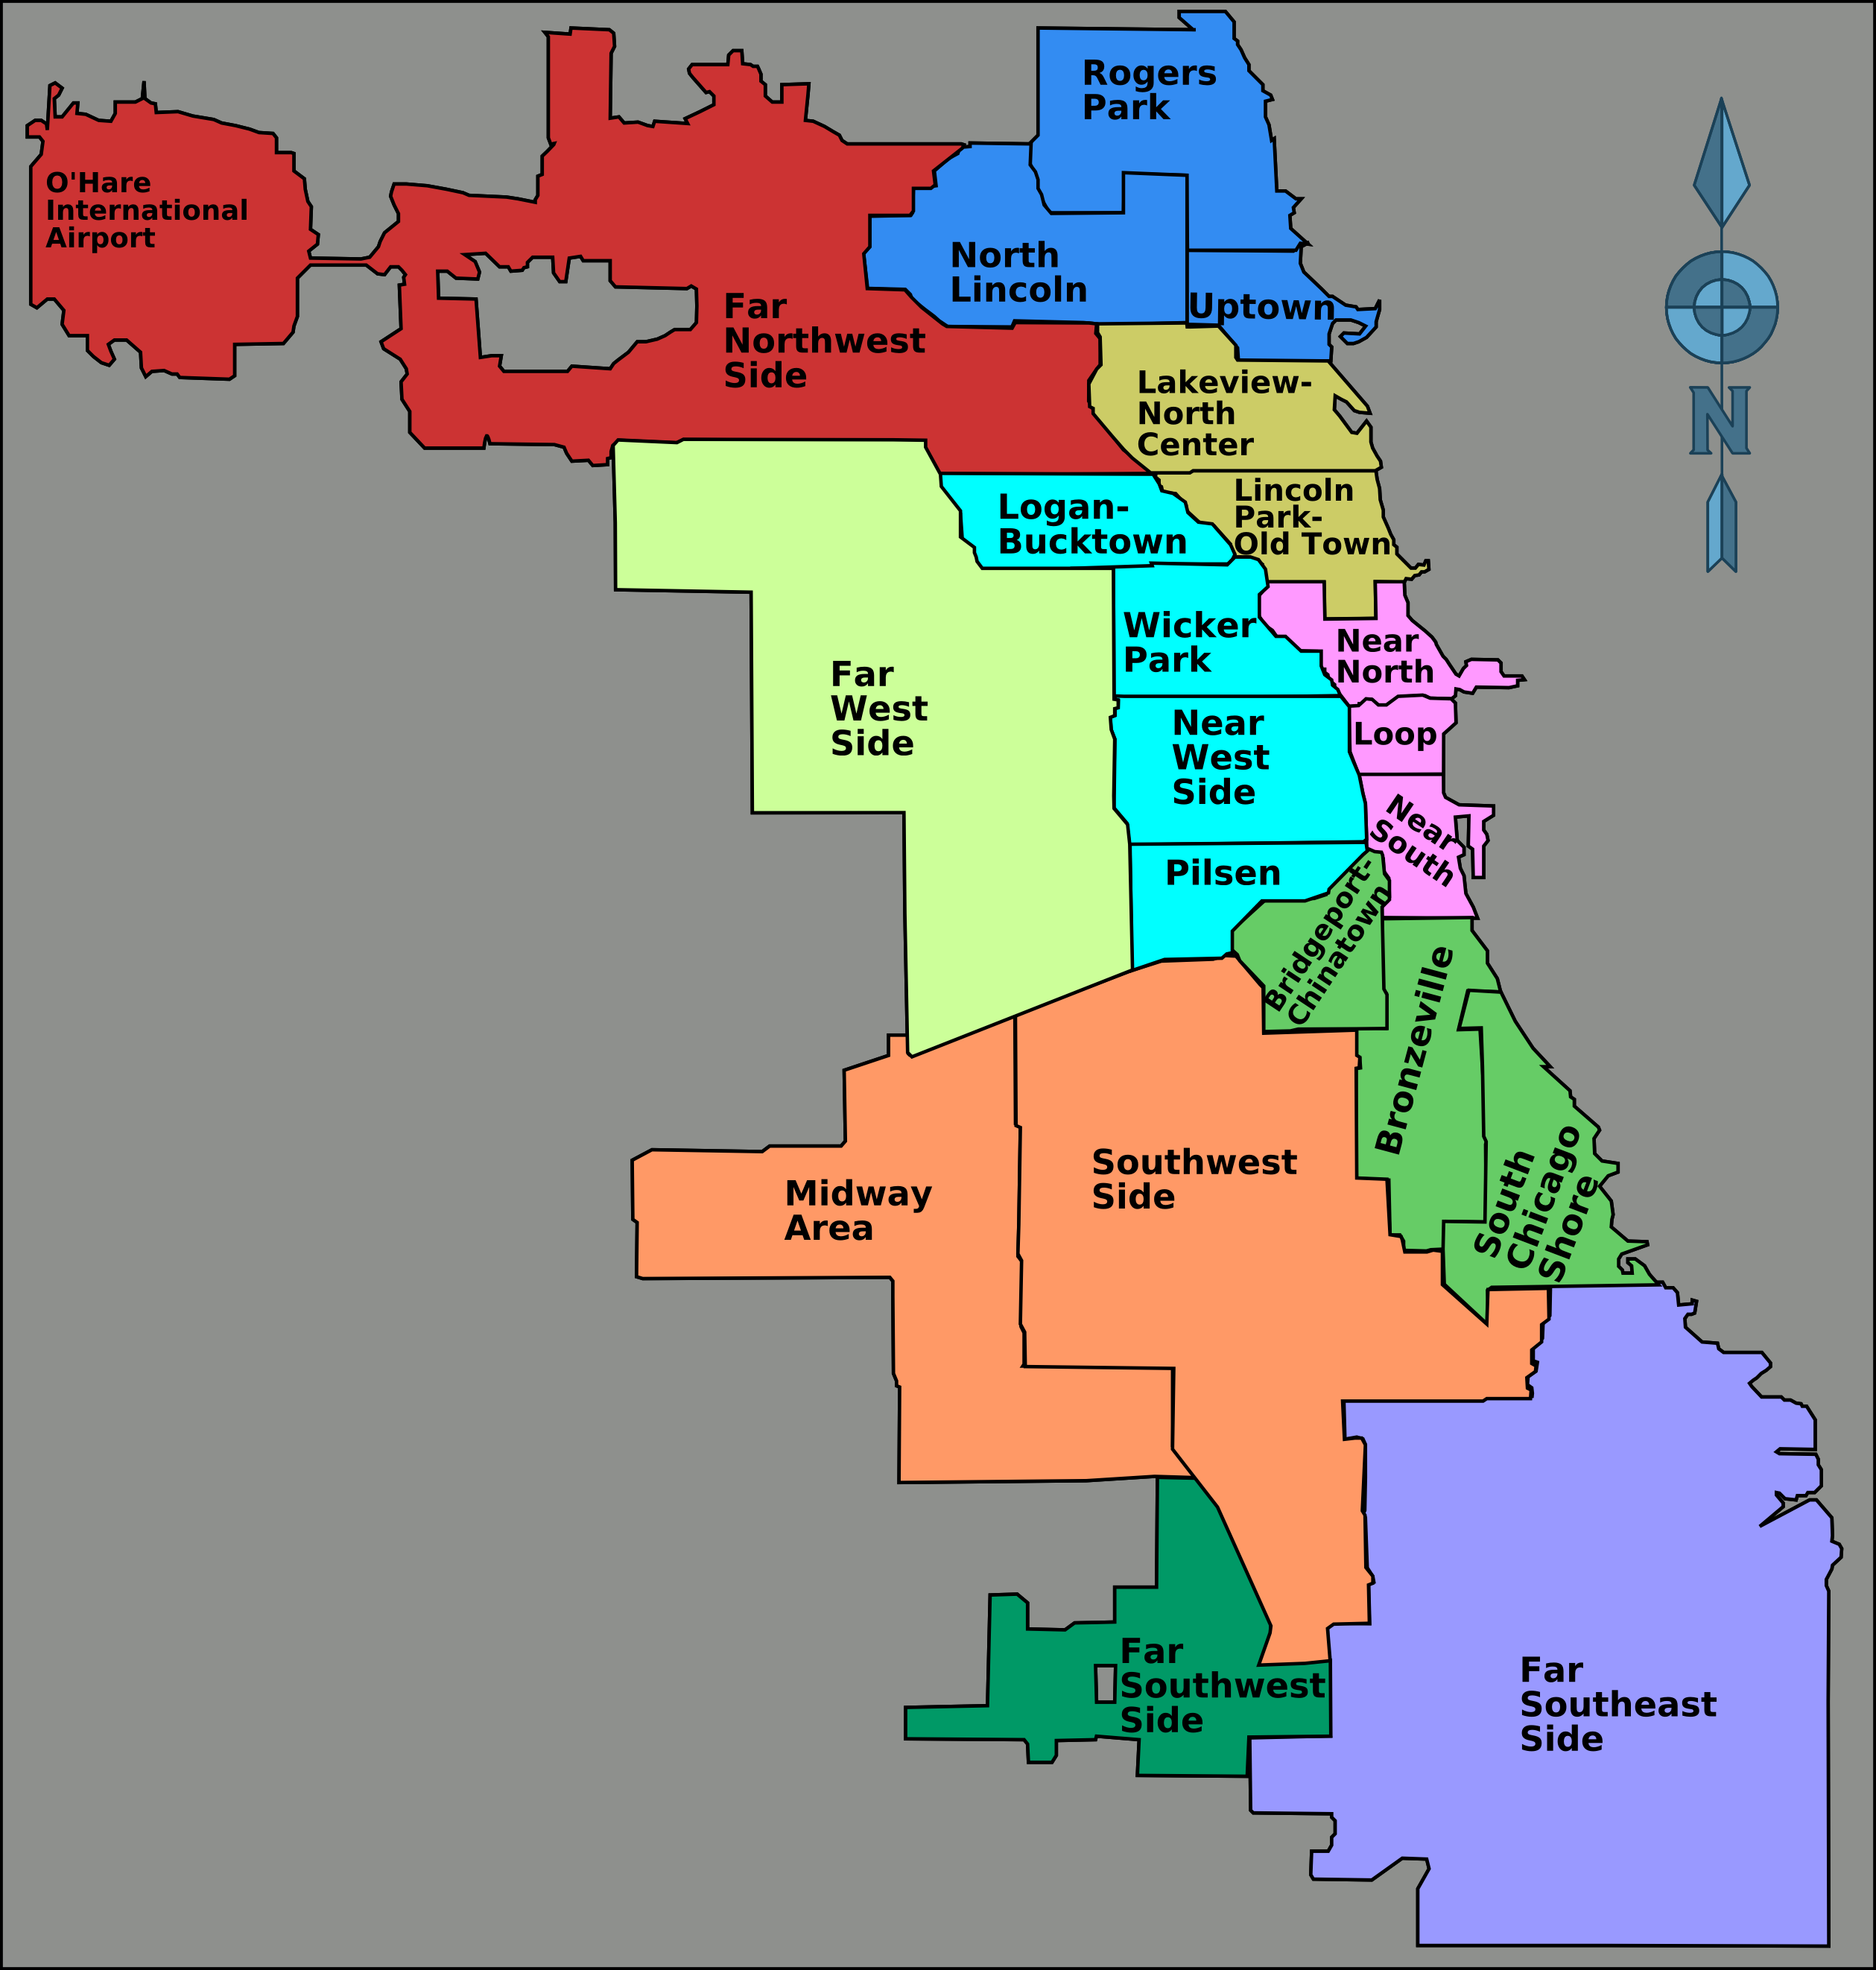
\includegraphics[scale=0.5]{chicago.png} \\
       2 millions d'habitants, Lac Michigan, Wisconsin au nord, l'Iowa et le Missouri à l'ouest, le Kentucky au sud et l'Indiana à l'est
	\section*{Illinois}
Villes principales:
\begin{itemize}
\item[Chicago]
\item[Aurora]
\item[Rockford]
\item[Naperville]
\item[Peoria]
\item[Springfield]: (capitale de l'État)
\item[Joliet]
\item[Moline]
\item[Evanston]
\item[Cicero]
\item[Decatur]
\item[East St. Louis]
\item[Bloomington-Normal]
\item[Champaign-Urbana]
\item[Rock Island]
\end{itemize}
La zone fut découverte par deux explorateur français Jacques Marquette et Louis Jolliet. Ils ont suivit le fleuve Illinois, C'est un ancien territoire Iroquois.
\chapter{La meute: BloodMill}
La meute fut créée par Wings avec l'aide des MoonWatchers. Il est naturellement devenu l'alpha.
D’abord Bulldozer (le juge) t’a rejoins, Trigger (l’éclaireur) vient ensuite. 
Finalement, Nocturne (la barman) et Scalpel (l’infirmière) sont arrivées.
Le territoire de la meute est tout Chicago à l'exception d'un quartier résidentiel au nord qui est sur le territoire des MoonWatchers. 
Le territoire comprend le quartier du loop, le south side, north Side, Bronzaville, les bords du Michigan.
\section{Le locus}
Le locus de la meute est un projecteur de cinéma. Il diffuse de l'essence du bonheur, joie et espoir. 
Le projecteur est localisé dans un vieux cinéma désaffecté du loop.
\subsection{Point Locus}
\begin{itemize}
\item[Trigger]:3
\item[Wings]:2
\item[Bulldozer]:2
\item[Nocturne]:2
\item[Scalpel]:2
\end{itemize}
\section{Le totem: Balbuzard pêcheur}
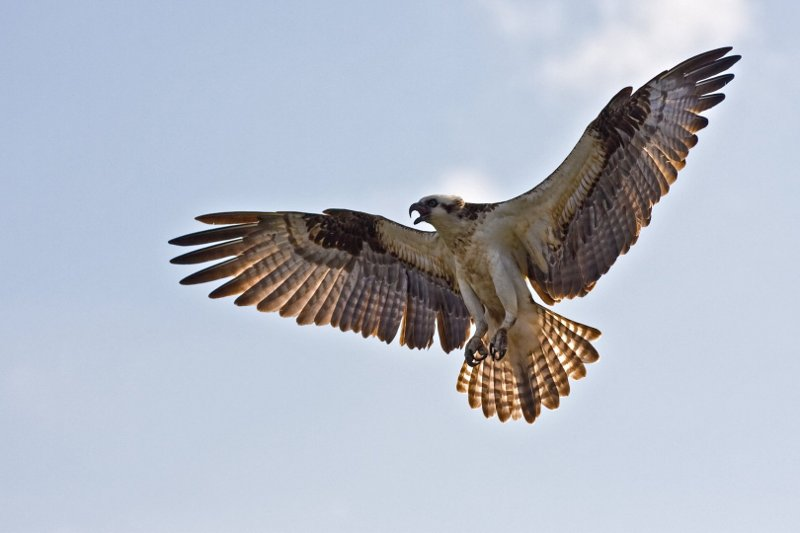
\includegraphics[scale=0.5]{totem.jpg} \\
C'est un rapace blanc tacheté de noir, il mange exclusivement des poissons.
l'interdit de la meute est l'obligation de manger du poisson cru et entier et Ne partager pas votre proie. Des reflets métalliques bornent ses ailes et ses serres.
\begin{itemize}
\item[Nom]: Yip Yip
\item[Concept]: Balbuzard pêcheur - esprit de la gloire
\item[Pouvoir]: 2
\item[Finesse]:5
\item[Résistance]: 3
\item[Volonté]: 6
\item[Essence]: 15
\item[Initiative]: 5
\item[Défense]:5
\item[Vitesse]:15
\item[Taille]:3
\item[Corpus]:6
\item[Influence]:Rapace: 2, Gloire 1, Prudence 1
\item[Bénédiction]: Vision Matérielle et Éclair
\item[Bonus] : +1 en Gloire et plus en vitesse pour Nocturne.
\end{itemize}

\subsection{Point Totem }
\begin{itemize}
\item[Trigger]:3
\item[Wings]:3
\item[Bulldozer]:3
\item[Nocturne]:4
\item[Scalpel]:3
\end{itemize}

\clearpage
\section{La cahalithe}
\begin{description}
\item[Nom:]{Lisy MacOrigan}
\item[Origine:]{Chicago}
\item[Auspice:]{Cahalithe/Visionnaire}
\item[Tribu:]{Griffes de Sang}
\item[Profession:]{Infirmière}
\item[Nom de guerre:]{Scalpel}
\item[Liste de dons]:Inspiration, Lune gibbeuse,Savoir,Force,Inspiration,Rage
\item[Age:]{17 ans}
\item[Histoire]{Tu es une fille de Chicago, issue d'un couple franco-américain. 
Ta mère était infirmière pendant la guerre, c'est ainsi qu'elle rencontra ton père.
C'était un soldat américain envoyé dans les tranchées afin d'évaluer la situation dans l'éventualité d'une intervention des USA. 
Il accompagnait une délégation d'officiers
américains. A la fin de la guerre, il retourna à Chicago avec l'amour de sa vie. 
Ta mère t'enseigna de petits trucs au fil du temps. Tu as une certaine expérience dans le domaine médical.
Tu aimes aider les autres. Tu as décroché un job dans un hôpital psychiatrique. 
Tu soignes les petits bobos du quotidien des patients certains sont des anciens combattants, d'autres des dépendants à l'opium et autres drogues. 
Les derniers sont des fous. Tu es très intéressée par les nouvelles pratique venue d'Europe.
La psychiatrie, le docteur H. Russel a suivi un stage pour soigner les soldats anglais et français qui furent traumatisés. 
Tu regardes cela avec beaucoup d'intérêt même si Hector te fait comprendre que ce n'est pas vraiment ta place.
Marie Dolovan est l'infirmière en chef, elle te supervise d'un œil patient et attentif. 
A ton arrivée dans l'hôpital Cook County de Chicago, tu as commencé à expérimenter des rêves étranges:
la lune scintillait d'une blancheur parfaite. Le monde que tu connais était plongé dans le noir.
Il n'y avait personne, tu te sentais prise au piège, poursuivie, observée voir même chasser. 
Dans un même temps, certains patients de l'hôpital se montrèrent très agressif envers toi. 
Jusqu'à cette nuit là, Jack Napier (les dents blanches), réussit à sortir de cellule.
Il t'avait tendu un piège, les portes des cages d'escalier étaient fermées, les alarmes désactivées, il joua avec toi. Il te poursuivit dans les couloirs. Il voulait
faire naître le désespoir en toi. Après t'avoir attrapé, il te coupa au niveau des cuisses, lécha ton sang. Il voulait te manger. 
Alors que tu étais prisonnière sous son poids, une force sortie de nulle part t'a envahi. 
Un appétit féroce naquit en toi. Tu le repoussas de toutes tes forces. 
A ta grande surprise, tu le projetas violemment contre un mur. 
Son apparence changea, il avait l'air plus fort et dangereux qu'avant. Tu te lanças dans la lutte sans aucun contrôle. 
La dernière image dont tu te souviens cette nuit là, c'est la peur sur son visage juste avant ton attaque. 
C'est ainsi que tu es devenue un Loup-Garou. La meute t'a recueilli et t'expliqua tout sur ta nouvelle condition.  
\\
Tu sais maintenant que les rêves que tu fais sont un don de mère lune. 
Tu ne les comprends pas toujours, mais ils sont souvent importants. 
Cela fait plusieurs jours que tu vois dans tes rêves une vaste étendue d'eau d'un calme étrange puis une nappe de feu vient recouvrir cette eau. Tu n'arrives pas à identifier les lieux.
\\
Depuis quelques jours, le service des urgences de l'hôpital t'a demandé de faire des gardes pour aider tes confrères face à la récente montée de violence qui provoque une suractivité à l'hopital. Il y a de nombreuses victimes de bagarres, des victimes d'agressions ou encore des problèmes liés à l'alcool. Cependant, l'ambiance n'est pas à l'inquiétude à l'hôpital.
Ce soir, c'est l'inauguration de nouveaux locaux pour le service de chirurgie. Tout Chicago est invité. En tant que membre du personnel, tu es convié à y participer. 
Le directeur de l'hôpital t'a dit qu'il faudrait être très gentille avec le maire (si tu voulais avoir de l'avancement). 

}
\end{description}
\clearpage
\textbf{\large Dons} 
\vspace{0.5cm}


\don{Eau Spirituelle}{Impose la crainte ou le respect}{}{1 point d'essence}{118}
\don{Déchirer le métal}{Il est plus facile de couper le métal}{Force + Artisanat + Gloire}{}{117}
\don{Hurlement primal}{Terrifie les ennemis}{Présence + Expression + Pureté (vs Calme)}{1 point d'essence}{134 }
\don{Coup Fracassant}{Les dégâts contondants deviennent des blessures létales}{}{1 point de volonté}{118}
\don{Cri de ralliement}{Redonne un point de volonté à ses alliés pendant la bataille}{manipulation + expression + Gloire}{}{119}


\clearpage
\section{Irraka}
\begin{description}
\item[Nom:]{ Edward Waltertown}
\item[Origine:]{Sud de l'Illinois}
\item[Auspice:]{Irraka/espion/Menteur}
\item[Tribu:]{Chasseur des ténèbres}
\item[Profession:]{Detective privée}
\item[Nom de guerre:]{Trigger}
\item[Liste de dons]:Discrétion,Évasion,Nouvelle Lune,Éléments,Modelage
\item[Age:]{31 ans}
\item[Histoire:]{Tu es un ancien flic qui a démissionné suite à une sombre histoire de policiers corrompus. 
Ils rackettaient des petits commerçants pendant les horaires de travail. 
Tu es parti avant qu'ils aient le temps de te mettre un de leurs sales coups sur le dos. 
Tu as démarré une carrière de détective privé. Cela te permet d'avoir des horaires assez libre en journée. 
Tu as acquis une assez bonne réputation à Chicago. Ton fait le plus célèbre reste le kidnapping de la fille de l'adjoint au maire. 
En réalité, elle était partie voir son petit ami, le jeune jardinier de la demeure familiale. 
Tu es convenu avec elle pour qu'elle raconte des actes héroïques à ton propos, elle a gardé 15\% de la prime. 
Des fois, les affaires ne se finissent pas aussi bien. Cependant, tu es devenu l'homme de main « classe » de la ville. 
Quand les hommes politiques veulent que cela avance, ils font appel à toi. 
La majorité de tes contrats sont le contrôle de maris ou d'épouses, ou encore la surveillance d'employés.
Tu es plus discret et compétent que la police de Chicago et beaucoup moins bruyant que la police fédérale. 
Il t'arrive de prendre une affaire intéressante gratuitement, pour faire une bonne action. C'est souvent des affaires qui n'intéressent pas la police.
Tu enquêtais sur la disparition de plusieurs petites filles dans un quartier pauvre de la ville. 
Tu trouvas la trace d'un groupe de la mafia italienne qui vendait les petites filles pour des clubs sur la côte ouest. 
Le transport des filles devait être effectué dans un train de marchandise, sous la mention: fleur de rose. 
Tu as fouillé en pleine nuit toute la gare, quand tu as finalement trouvé le bon, tu as été repéré et sonné. 
A ton réveil, le train venait juste de partir.\\ 
Encore visible au bout de la gare, tu n'as pas compris pourquoi une voix en toi te disait que tu pouvais le faire. 
Tu pouvais te libérer et rattraper le train. Tu as couru le plus vite que tu aies pu. Tu sentais l'odeur des filles apeurées. 
Tu as sauté sur le wagon de queue et tu as massacré tous les hommes en armes. C'est ainsi que tu es devenu un loup-garou. 
Quelques jours plus tard, des gens se sont présentés à toi pour t'expliquer ta nouvelle condition et les obligations qui viennent avec elle.
Tu as fini par intégrer leur meute.
Tu prends ton travail encore plus au sérieux maintenant que tu sais ce qui se cache dans l'hisile (le monde des esprits).
Depuis quelques jours, tu as remarqué une montée assez étrange de la violence dans les quartiers chauds. De nombreuses bagarres dans des bars mais aussi en pleine rue ont éclaté sans aucune raison. Le nombre de mort suspecte est en augmentation. Tu penses que la meute devrait peut-être faire attention à ça.
\\
Ce soir, le maire t'a invité au gala d'inauguration du tout nouveau service de chirurgie de l'hôpital Cook County. 
Officiellement, tu es là en tant qu'ami du maire. 
En réalité, tu assures sa sécurité et laisse traîner tes oreilles pour écouter un peu les ragots pour lui. 
Ta meute est au complet dans cette soirée. 
C'est un peu inhabituel comme lieu de rencontre, mais au moins tu espères que la soirée ne sera pas trop ennuyeuse. }
\end{description}
\clearpage
\textbf{\large Dons} 
\vspace{0.5cm}


\don{Ombre mouvante}{}{}{1 Point d'Essence}{115}
\don{Poudre aux yeux}{}{Manipulation + Subterfuge + Honneur (vs Calme + Instinct Primal)}{}{111}
\don{Double sens}{Terrifie les ennemis}{Intelligence + Investigation + Gloire}{ 1 point de volonté}{111}
\don{S'esquiver}{Se libérer de liens (menottes, camisole...)}{}{1 point de volonté}{132}
\don{Distraction}{}{Manipulation + Subterfuge + Gloire (vs Résolution + Instinct Primal) }{}{133}



\clearpage
\section{Rahu}
\begin{description}
\item[Nom:]{Peter Alington}
\item[Origine:]{New York}
\item[Auspice:]{Rahu/Guerrier}
\item[Tribu:]{Maitre du Fer}
\item[Profession:]{Aviateur/héritier}
\item[Nom de guerre:]{Wings}
\item[Liste de dons]:Domination,Force,Pleine lune,Modelage,savoir, technologie.
\item[Age:]{35 ans}
\item[Histoire:]{
Ancien pilote de chasse dans l'armée américaine, tu es maintenant un pilote de voltige. Tu as ouvert une petite école de pilotage à Chicago. 
L'essentiel de tes clients sont des jeunes millionnaires ou des gens qui désirent s'embarquer dans quelques expéditions dangereuses (les pôles etc.). 
Tu es l'instructeur personnel du fils du maire. 
Cela fait 10 ans que tu as ouverts cette école, tu as eu quelques décès pendant les entraînements, mais bien en dessous des taux des écoles militaires ou de tes concurrents. De fait, elle commence à avoir bonne réputation.
Il est vrai que tu inspectes les avions avec beaucoup de minutie. Il est très difficile de garder son poste de mécanicien chez toi. 
Cependant, tu penses avoir trouvé les bons. Les avions commencent à être vraiment robustes. Tu as hélàs de moins en moins le temps de piloter pour le plaisir
entre tes obligations pour maintenir à flots ton entreprise, les courts et les voltiges pour les films. Malgré la crise, ton affaire prospère. 
\\
Il y a quelques temps, tu as reuçu un nouvel avion: un « Beechcraft Staggerwing ».
Tu as voulu effectuer le premier vol. 
Après plusieurs heures de vol et sans aucune raison, l'avion a eu une panne de moteur au-dessus des grandes plaines au sud de la ville.
Ton expérience t'a permis de te poser en douceur dans un champ. Ta radio ne semblait pas fonctionné. 
	Tu t'es très vite senti observé. Des odeurs particulièrement fortes autour de toi.
Un sentiment de danger t'a envahie, tu entendais des hurlements de loups partout autour de toi. Grâce à ton expérience, tu t'es préparé  à recevoir tes invités. 
Quand l'assaut fut donné, une envie de survie et une rage profonde a libéré une chose en toi. 
A ton réveil, il y avait trois corps humains autour de toi. Tu étais sévèrement blessé. 
Tu as pu regagner la civilisation après quelques heures de marche. Un médecin t'ausculta dans le petit village de Farmington 
Il te questionna un certain temps, il pensait que tu t'étais soigné au fer chauffé à blanc, dans tous les cas, il n'avait jamais vu de telles blessures. 
Deux jours plus tard, un groupe d'individus vint te remercier pour la destruction de la meute "Crocs dentés" une meute de purs. 
Grâce à la destruction de trois des quatre membres la meute, ils ont pu finir le travail en attaquant le chef (ils avaient une dent contre cette meute). 
Ils voulaient connaître le nom de ta meute. Devant ton incompréhension, ils se sont rendus compte que tu étais un nouveau né. 
Ils t'ont alors expliqué ta nouvelle condition et ses obligations. Tu as créé ta meute dans Chicago avec leur conseil. 
D'abord  Bulldozer (le juge) t'a rejoint, Trigger (l'éclaireur) vient ensuite. Finalement, Nocturne (la barman) et Scalpel (l'infirmière) sont arrivées. 
\\
Le maire de la ville t'a invité à participer à la grande inauguration du nouveau département de chirurgie de l'hôpital Cook County. 
Tu n'as pas envie d'y aller mais bon il donne beaucoup d'argent à ton école. Il va se servir de ton image de héros de guerre. Tu t'es arrangé pour que tous les membres
soient là. Ce sera moins pénible probablement.   
}
\end{description}
\clearpage
\textbf{\large Dons} 
\vspace{0.5cm}


\don{Coup Fracassant}{Les dégâts contondants deviennent des blessures létales}{}{1 point de volonté}{116}
\don{Armure de Rage}{}{Vigueur + Survie + Honneur}{1 Point d'Essence}{138}
\don{Étreinte de mort}{}{}{1 Point d'Essence par morsure}{111}
\don{Redresser}{}{}{1 Point d'Essence}{132}
\don{Trahison du métal}{}{Astuce + Artisanat + gloire}{}{146}



\clearpage
\section{Elodothe}
\begin{description}
\item[Nom:]{Christopher Holabird}
\item[Origine:]{Boston}
\item[Auspice:]{Elodothe/juge}
\item[Tribu:]{Seigneur des tempêtes}
\item[Profession:]{Architecte}
\item[Nom de guerre:]{Bulldozer}
\item[Liste de dons]:Demi lune, Perspicacité,Protection,Domination,Évasion,Météorologie
\item[Age:]{28 ans}
\item[Histoire:]{
Ton grand-père et ton père (William Holabird) sont de grands architectes, ils ont construit de nombreux bâtiments à Chicago. 
Leurs personnalités te font un peu de l'ombre dans la profession.
Par chance, tu travailles dans le cabinet d'architecture familial, ce qui te laisse la possibilité de faire un peu ce que tu veux de ton temps. 
Tu es content, car la construction du nouveau département de chirurgie de l'hôpital Cook County est maintenant terminée.
L'inauguration, c'est ce soir, tu as hâte d'y être. 
C'est ton grand jour de gloire. Ce sera sûrement ton dernier travail, tu préfères te concentrer sur ta nouvelle vie de loup-garou.
\\
Un soir alors que tu cherchais de l'alcool pour une petite soirée privée que tu organisais afin de séduire plusieurs jeunes femmes séduisantes. 
Tu as passé deux ou trois coups de téléphone pour avoir des adresses. 
Tu as finalement trouvé un point de rendez-vous dans le \textit{South Side} de la ville. 
Hélas, des petits malfrats t'avaient tendu un piège pour te braquer tout ton argent. 
Tu ne t'es pas laissé faire, mais ils étaient bien trop nombreux pour toi et bien trop équipé. 
Ils t'ont fait un passage à tabac en règle. Alors qu'ils s'apprêtaient à te partir et te laisser pour mort, tu as vu le reflet de la lune dans ton propre sang. 
Tu t'en souviens encore maintenant, c'était une demi-lune parfaite. Il t'a semblé voir un visage. 
Une chaleur nouvelle envahie tout ton corps. Une vague de rage parcourue ton échine. 
Bizarrement, la douleur avait disparu, tu voulais te prouver que tu pouvais réussir un truc. Le reste te semble flou. 
Tu te souviens t'être réveillé, nu au milieu de trois cadavres humains. 
Tu es rentrés chez toi discrètement à l'aube, avec des vêtements pris sur les corps. 
Les corps des trois malheureux ne furent jamais retrouvés. Tu reçus la visite de Wings (le guerrier) qui t'expliqua un peu ta nouvelle condition et ses obligations. Il te proposa de rentrer dans sa meute et il ne te laissa pas beaucoup le choix.
Puis ensemble vous avez cherché Trigger pour le faire rentrer dans la meute. Enfin vous avez dernièrement été rejoins par Nocturne et Scalpel.
}
\end{description}
\clearpage
\textbf{\large Dons} 
\vspace{0.5cm}


\don{Aura de trêve}{}{Manipulation + Persuasion + Honneur}{}{113}
\don{Gelée Mortelle}{}{Manipulation + Survie + Honneur}{}{124}
\don{Écho Onirique}{}{Astuce + Investigation + Honneur}{}{136}
\don{Sentir la malice}{}{intelligence + Empathie + sagesse}{}{135}
\don{Poudre aux yeux}{}{Manipulation + Subterfuge + Honneur}{}{111} 



\clearpage
\section{Ithaeur}
\begin{description}
\item[Nom:]{Rose Baker}
\item[Origine:]{Chicago}
\item[Auspice:]{Ithaeur/Shaman}
\item[Tribu:]{Os de l'ombre}
\item[Profession:]{Barman}
\item[Nom de guerre:]{Nocturne}
\item[Liste de dons]:Croissant de lune,Élément, modelage,Mort,Perspicacité,Protection
\item[Age:]{19 ans}
\item[Histoire:]{
Tu es une jeune fille noire vivant dans le quartier de "Bronzeville". Ta mère travaille dans les usines automobiles de la ville. Elle a quatre enfants (de quatre pères différents). Tu as un grand frère et deux petites sœurs.
Tu vois l'état de santé de ta mère se dégrader au fil du temps, tu as tout fait pour éviter ce même destin. Préférant le monde de la nuit où l'argent coule à flot. \\
Au réveil après une soirée clandestine, où tu avais travaillé comme barman. 
Ton cachet de la nuit avait disparu. Tu as compris tout de suite que \textit{Ernest} (ton grand-frère), était le coupable.  
Tu as essayé de savoir où il est allé en questionnant des jeunes du quartier.
Tu as pu retrouver sa trace dans un entrepôt (hangar N°18) près du port sur le lac Michigan. Des gros bras t'ont vu et t'ont amené à l'intérieur, ton frère était prisonnier. Ils t'ont jeté dans une cuve vide en "attendant le patron".
Tu as entendu la conversation entre ton frère et le "patron". 
Il avait visible une grosse dette financière avec l'organisation. 
Il a essayé de négocier un délai supplémentaire. Le "patron" a évoqué l'idée d'utiliser tes avantages naturels pour rembourser la dette.
ton frère a voulu s'y opposer. Le patron ordonna à ses gros bras de te conduire dans un bordel du sud de la ville.
Ton frère s'est interposé, mais tu as entendu un coup de feu partir. 
Tu as littéralement pété un câble. La cuve parue plus étroite d'un coup, tu te souviens avoir essayé de sortir de la cuve.


Après cette sensation, tu ne te souviens plus de rien. À ton réveil, tu étais dans le hangar, il y avait cinq corps autour de toi, tous horriblement mutilés. 
Tu étais nue et il faisait froid. Tu fut alors aidé par trois hommes: Wings (le guerrier), Trigger (l'éclaireur) et Bulldozer (le juge).
Ils t'expliquèrent ce qui s'était passé. Tu venais de vivre ta première transformation. La cuve ressemblait plus à un choux-fleur qu'à autre chose. Malheureusement tu as compris par la même que tu avais tué ton frère. Tu te juras de ne plus jamais perdre le contrôle comme ça. 
L'intégration dans la meute fut salvatrice. Tu t'es découvert pleins de nouveaux talents et tu as recherché quelques informations sur ton passé.\\
Sur le plan professionnel, il y a du mieux. Les membres de la meute sont assez influent à Chicago, tu fais des contrats beaucoup plus lucratif et moins risqué: Cocktail à l'école d'aviation ou Soirée pour le cabinet d'architecture. 
Ce soir, tu seras responsable du bar au gala d'inauguration du nouveau service de chirurgie du Cook County Hospital. Contre toutes attentes, tu as été sélectionné.  
Il va y avoir du beau monde. \\
Une série de bagarre générale a éclaté dans les grands speakeasies de la ville. De nombreux gens du métier (barmans, serveuses et vigiles) ont été agressé. C'est une bonne chose pour toi et tes affaires. Tout le monde dans le milieu pense que c'est un coup des Irlandais pour faire pression sur les autres speakeasies.

La cérémonie a lieu ce soir. Tu t'es donc présentée à l'avance. \\
Barney Groover t'a expliqué un peu le deal pour la soirée (C'est l'organisateur, le bras droit du directeur de l'hôpital). 
Bien que mal à l'aise de parler avec une négresse, il t'a montré le bar et les alcools: Bières de basses qualités (légal), du whiskey (illégal) de très 
mauvaise qualité (tu n'en donnerais pas à un chien). C'est probablement de l'alcool frelaté (alcool de bois avec de l'huile de moteur pour la couleur) et le dernier est un rhum qui est particulièrement de bonne qualité.
Il est réservé qu'à certains membres, le mot de passe est "Érable", ils viendront uniquement vers toi. Il est peu probable que tu en serves beaucoup. 
Les autres barmans sont des employés de l'hôpital, ils ont du mal à te faire confiance. Ils ne te semblent pas très compétent non plus.\\

Le point positif c'est qu'il y a peu de chance de voir les Irlandais, ce soir. Même si une bagarre éclate, tu sais que toute ta meute sera là.
}
\end{description}
\textbf{\large Dons} 
\vspace{0.5cm}


\don{Témoignage d'un cadavre}{}{Manipulation + occulte + Pureté}{}{129}
\don{Oeil sur les deux mondes}{}{Astuce + occulte + Sagesse}{}{104}
\don{Manipuler la terre}{}{Dextérité + Artisanats + Ruse}{1 point d'essence}{108}

\textbf{\large Rituels} 
\vspace{0.5cm}

\don{Rite Funéraire}{}{Harmonie}{}{151}
\don{Invoqué un esprit}{}{Harmonie}{}{152}
\don{Pierre consacrée}{Stocke de l'essence dans un objet}{Harmonie}{}{150}
\don{Renforcer les marches}{Augmente ou diminue le Goulet (frontière entre les deux mondes)}{Harmonie}{}{154}




\chapter{L'histoire commence}
\section{Les préparatifs}
Le scénario comment Nocturne et Scapel sont déjà dans la place.
Les musiciens sont en train de se préparé. Les gens commence à arriver. 
Trigger arrive.
Un homme noir s'acoude au contoir et commence un jus de mangue. Il est musicien, il remercie la petite et se casse.
Devant les journalistes/photographes Wings et le Maire sont acceuillis par Bulldozer. 
\section{La cérémonie}
Les Pj sont à la soirée d'inauguration du nouveau service de Chirurgie. 
Le maire n'a pas peur il a invité la grande chanteuse de la nouvelle Orléans :Marie " Belle-voix" Coccinelle. Elle est accompagnée par un jeune trompettiste: Louis Amstrong.
La fête va bon train, une partie des invités s'éclipsent vers d'autres partie du bâtiment.

Les Pj restent dans le hall principal. Certains invités ont apporter leur alcool maison.
Les alcools disponibles sont : De la bière seringué, du Whiskey caramel et du gin. Un traitement spécial est fait pour le rhum. Probablement le seul alcool de qualité (Il vient de Martinique).

Rose "Nocturne" Baker reçoit des commandes de tout cependant le rhum est réservé au membres bienfaiteur.
Il faut un mot de passe mais globalement toutes les demandes sont gérées par l'intendant Barney Groover. 
Il est probable que beaucoup de monde est du mal à parler avec une negresse.
Barney (Il travaille pour l'hôpital) vient récupéré une grosse quantité de rhum pour les vip du salon privé. 


\section{Un vampire alcoolique}
le salon privé est en faite un bordel pour la nuit organisé dans les nouvelles chambres de l'hôpital.
Le maire y invitera Lisy "Scapel" pour des petits plaisirs personnel. Des amis du maire sont là. Parmi eux se trouve une poignée de vampire:
Un homme jeune : 24 ans, jeune vampire très élégant mais semble transparent. Il est l'ombre de son chef.
Une jeune fille de 16 ans: Alice, c'est la plus vieille des vampires, elle est la plus grande opposante au prince de la ville (il n'est pas là). 
Elle se cache derrière la cours du primogène Nosferatu et patron de la Coterie: Les gastronomes pour se protéger.
Elle pousse le fauteuil roulant.
Charles: Un homme d'environs 50 ans, il est dans un fauteuil roulant. Il est le primogène Nosferatu et patron de la Coterie: Les gastronomes.
+ 2 autres, des gardes du corps. 

Une personne ira demandé du rhum, il boira verre sur verre, au bout d'un momemt Nocturne n'en aura plus.
L'homme lèvera le ton, puis sa femme viendra le chercher pour danser. Il reviendra à la charge en cassant la gueule a un barman ou server. 

Dans la zone vip, le rhum coule à flot.
L'ensemble des buveurs de rhum en demande encore et encore. L'intendant a du mal à suivre.
Un vampire enfermé dans une chambre (le jeune) avec 2 hôtesses deviendra fou et aura bu tout le sang des hôtesses.

La raison est simple, Le rhum est empoisonné d'essence addictive ( avec un regard sur les deux hommes, on peut distingué un hameçon dans le verre dans un liquide noirâtre).
Le vampire est devenu fou à cause de la puissance du breuvage. Les humains normaux peuvent boire de l'alcool mais les vampires doivent boire le sang de personne sous ivresse. 
Le vacarme provoqué par le vampire est audible pour les loup garous (test de perception-3: bruit du concert).
s'ils échouent, il sera facile de voir les bras droits des différents mafieux aller dans le salon privé (en réalité se sont quelques goules des vampires). Le vampire aura été maîtrisé par un de ses semblables mais les humains commenceront à ressentir la manque et deviendront agressif.
Le vampire nommé Alice dira aux PJ  (s'ils n'ont pas compris) que l'alcool semble être responsable mais elle n'y trouve rien de spécial dedans. 

Alice est une mehket. Elle aura pu voir la scène gârce à ses dons d'auspex. Les PJ peuvent la voir faire une transe entouré du cadavre des deux hôtesses.
Elle s'est installée à la place du coupable dans la chambre qui le lieu du crime. 


\section{Effet de la consomation de Rhum sur un Uratha}
si des LG goutent l'alcool, leur essence commence a être pollué. 
Il doivent faire un (jet de volonté- le nombre de verre consommés) pour résister au manque, si échec il recommande un verre. 
S'il n'y a plus d'alcool, ils doivent faire un jet de volonté.
Si echec transformation en forme gauru (puis test de rage mortelle). 

\section{Rhum}
La raison est simple, Le rhum est empoisonné d'essence addictive ( dans l'ombre, on peut distingué un hameçon dans le verre dans un liquide noirâtre).
L'écho de l'essence est très jouissif mais sombre. 

\section{D'où vient le Rhum ?}
Pour avoir des informations sur la provenance du rhum, seul l'intendant Barney de l'hopital est au courant. Attention, il peut être une victime de la folie alcoolique des VIP. A la discretion du MJ. S'il est vivant, il apprendra au PJ que c'est un certain: Joe "Brook" Ulster qui lui a vendu cet alcool (ainsi que les autres). 
\section{Le revendeur }
Joe fournit la ville entière, il a du rhum et d'autres alcool de moindre qualité. 
Il sera très méfiant, il faut le trouver de façon très délicate. Rendez-vous dans un lieu dont il a la maitrise.
C'est un personnage assez petit, excité et méfiant, voir parano.
Il est très méfiant car plusieurs personnes ont essayé de lui piquer sa marchandise. Il est marqué par des blessures. Mais ils ne s'occupent que de grosse quantité. Le détail est fait par des petits dealers dans les quartiers.
Il ne connait pas le fabriquant  mais il aime beaucoup ça lui rapporte beaucoup.

Il est sur nouvelle affaire, du rhums de Saint pierre et Miquelon. Il est livré par des Rhum runners sur le lac Michigan. Il partiera assez rapidement car il faut justement qu'il prépare la nouvelle livraison.
\section{Les Rhum runners et incendie sur le Lac}
Si les Pj se trouvent au bord du LAC ou qu'il suivent le revendeur longtemps. Ils pourront assister à la livraison d'une cargaison de rhum. 
Les nouvelles livraisons se font sur le lac Michigan, les bateaux sont de petites embarcations mais très rapides. La grosse livraison sera détruire par l'action de l'esprit de l'addiction et ses sbires.


\section{le monde des esprits}
Le monde des esprits en vraiment en bordel, il y beaucoup d'esprit de la violence, mitrailleuse, de la corruption et de l'addiction/ivresse.

Si les Pj entre en contact avec un esprit, ils apprendront que les esprits sont effrayés par un esprit tres puissant qui s'approche: Magathe.
Ils se sentent observer, cette sensation disparait s'ils cherchent d'ou cela vient.

\section{Pendant la cérémonie}
Pendant que les PJ sont à la soirée, une enorme émeute éclate entre deux gangs à l'intersection d'une rue de bronzeville.
Elle est le fait de possédés qui ont déclancher la violence. L'intersection contient un tas d'ordures car il y a une greve des services de ramassages.
C'est un locus. il se situe au-dessus d'un des nids de Beshilus.

\section{Les brasseries clandestines }
Le rhum est fabriqué dans divers endoit plus ou moins proche du Loop (centre ville de Chicago). ce sont souvent les égouts qui sont utiliser pour dissimuler les odeurs et les travailleurs. 
Chaque labos est aussi un locus qui déverse une essence de la corruption/l'addiction. Les loup-garous doivent se poser plusieurs questions:
Est-il normal de trouver des locus si nombreux dans leur territoire, et l'esprit nourrissant ces sources est clairement très puissant plus puissant qu'eux (il faudra rusé pour l'avoir). 

\section{Informations récupérable dans la presse}
    \subsection{Locale}
        La convention démocrate nationale de 1932, ou Franklin Delano Roosevelt invoque son programme contre la crise "le New deals" il devient officiellement le candidat du partie. La convention débutera le lendemain de la cérémonie del'hopital.  
        L'émeutes à l'angle de north Clark Street et willow street 
        La cérémonie d'inauguration de l'hopital avec le maire et les joueurs. 

    \subsection{Nationnale}
        L'incendie spectaculaire de port de New York, qui n'a fait aucune victime mais beaucoup de dégâts matériels. Il a eu lieu près du navire le SS Gabrielle 
        le navire de l'expedition StarkWeather. 
    \subsection{Internationnale}
        La monté du faschisme en europe. La guerre d'espagne.

\section{Les possédés }
Les gens qui travaillent à la fabrication du rhum sont de véritables pantins, regards globuleux, ils seront agressif vers les PJ. 
Il est possible que la destruction des brasseries artisanales soit le plan pour affaiblir l'esprit. 
Ou bien, les pour une raison où une autre. 
Les loup garou peuvent effectuer un test de perception pour sentir une odeur.

\section{Cendre dans les égouts}
    Il est possible qu'Alice soit en difficulté, et recroise la route des PJ. 
Elle les informera que des évènements étranges se passe dans les égouts. 
Les hommes de main de Charles n'ont pas donnée de signe de non-vie depuis un certain temps. 
Le prince soupçonne des diableries qu'elle aurait faite car même des soldats du prince sont morts dans les égouts. 
Elle a senti la même odeur que celle du rhum. 
Si les PJ fouillent les égouts Alice pourrait vouloir les suivre. Ils seront entourer de bruit de rats. 
Une énorme quantité de rats tourne autour d'eux. Il est possible de détecter la présence d'esprit de la tristesse et de la peur.
Les rats peuvent parler avec les PJ. Ils les conduiront vers un couloir étrange ou l'odeur de la mort est présente. 
Dans le couloir, il y a deux tas de cendre et des centaines de rats morts. 
Les joueurs pourrons identifier qu'il y avait clairement deux camps.
Les vampires était escorter par des goules animales. Elles se sont battues pour protéger leur sir. 
En face, les Beshilus ont protéges leur territoires. Ils ont tué les deux vampires. Dans les rats mort il y a clairement des traces de 
combats entre rats.


\section{Les hommes rats}
L'odeur leur semblera familière mais il ne la connaissent pas, elle leur rappelle un mauvais souvenir au fin fond de leur mémoire. 
Ils devront aller plus profondément dans les égouts.
Ils entendront le bruit de pas des dizaines dans le profondeur des égouts. Ce sont des Beshilus. Ils vivent dans les égouts de Chicago. Sans le vouloir, il facilite le travail des esprits, le goulet est une vrai passoire.
Il est très facile d'outre passer.
Il est probable que les PJ souhaitent les détruire, les combats sera fait alors. 
Dans le cas contraire, il peut être intéressant de voir les Beshilus dans s'approcher et mettre en danger le locus de la meute.
A noter, qu'être proche du locus ne provoque plus les mêmes effets qu'avant. En effet, les loup garous ne sentiront que peu de différence entre le reste de la ville et 
la proximité du locus. Il peut être intéressant de jouer la dessus. Les joueurs penseront peut-être que le locus est endommagé...

Il est important de comprendre que les Beshilus n'ont aucun rapport avec les possédés et autres fait étranges ces derniers temps. Leur travail facilite grandement le
travail des esprits et une quantité phénoménale d'essence passe par le monde des esprits. Des choses exilés aurait peut-être dur le rester.


\section{Les esprits}
Il y a deux principaux esprits qui influencent grandement le territoire de la meute. 
Le premier est un esprit de l'addiction, il est le réel danger immédiat.
il possède une technique qui lui permet de convaincre facilement les accros, d'exécuter telle ou telle action. 
Ainsi il aura pris le contrôle de divers humains pour la fabrication de son rhum addictif. 
Grâce à l'alcool, il aura un vampire sous ses ordres et 3 loup garou de la meute voisine (ils sont connus pour avoir un penchant pour la boisson). 
Ils seront sa garde du corps personnels le combat pourrait avoir lieu dans le monde des esprits. 

Le deuxième esprit plus puissant encore mais moins dangereux sur le moment est l'esprit de l'argent. Son désir est que l'argent soit désiré et en activité.
Il souhaite que l'argent circulent, il a ainsi convaincu l'esprit de l'addiction de l'aider dans sa tâche. 

La quantité d'essence est telle qu'elle va attiré certainement des choses qu'il aurait mieux-value oublié. Un esprit banît du passé.

 
\section{Un mago}
L'argent collecté par le commerce du rhum ne sert à rien à l'esprit de l'addiction. L'esprit de l'argent l'aura poussé a redistribuer cet argent.
Les SDF des ghetto de Chicago reçoivent de l'argent, qu'ils vont boire.
De grosses quantités sont jouées aux courses, combat de chiens, combat de boxe. L'argent doit circuler.
Il est possible de retrouver une quantité importante d'argent dans les brasseries clandestines.  

\section{La meute voisine: les MoonWatchers}
Meute voisine, elle a un énorme territoire mais il semble en jachère s'est temps si. 
Meute possédant un territoire très vaste autour de Chicago. Son territoire est principalement constitué de la campagne environnante.
Elle surveille un seul quartier de Chicago. 
Les PJ se rendrons compte que le territoire de la meute est bien plus endommagé que le leur.
Ils sentiront forcement que le territoire est à l'abandon. 
S'il enquête la dessus, il trouverons le corps de l'alpha de la meute clairement mutilé et même manger. 

L'alpha est mort, c'était un Elodothe: Jack "Dents blanche" Arron.
Le cahalite: Os-dur (William Asperd) : Force 3 (4/6/5/3), bagarre 3
Le irraka: Sauvage (Charles Edmonth): Force 3 (4/6/5/3), bagarre 1
Le irraka: Silence  (Helen Carpenter) : Force 2 (3/5/4/2), bagarre 4
\section{Attentat sur le futur président}
Franklin Delano Roosevelt est candidat aux élections présidentielles de 1932. Il est actuellement en campagne électorale. 
Il souhaite passer par Chicago pour apporter son soutien au candidat pour la mairie et présenter son programme. 
Notamment la fin de la prohibition et la relance économique par l'investissement massif de l'état dans de grands projets.
Il est fort probable que les sbires de l'esprit de l'addiction l'attaque pour protéger leur business.
Les PJ pourrait apprendre des informations sur la préparation de l'attentat. Trouver des plans et descriptifs des procédures de sécurité 
pour le discours de campagne au bord du lac Michigan. 

\section{Schéma directeur des Esprits}
Esprit de l'Argent 	-> Esprit de l'addiction	-> Contamination des bouteilles de rhum 	-> Possession et influence sur humains
(feu)			-> Esprit de la Violence	-> Destruction des concurrents			-> Idem facilité par le travail des hommes-rats

Hook Fisher essaie d'invoquer un Idigame, il lui faut pour cela un bon nombre d'influencé ou de possédés. Ils travaillent à affaiblir le goulet avec ses "hommes". C'est pour cela qu'il prévoit d'assassiner le président. Il cherche à réunir le maximum de gens dans un hangar (du port) pour qu'il participe à un rituel. 
\section{Caractéristique des esprits}
\subsection{L'esprit de l'addiction}
\begin{itemize}
\item[Nom]: Hook Fisher
\item[Concept]: Esprit de l'addiction (Jagglings majeur)
\item[Pouvoir]: 11
\item[Finesse]:12
\item[Résistance]: 10
\item[Volonté]: 20
\item[Essence]: 25
\item[Initiative]: 24
\item[Défense]:12
\item[Vitesse]:15
\item[Taille]:6
\item[Corpus]:16
\item[Influence]: Pantin: 4, Bois 5, Addiction 5, Alcool 5.
\item[Bénédiction]: 
\item[Interdit]: Ne se nourrir que de son travail. S'il reçoit de l'essence par don, il perd le double en point d'essence (à l'exception d'un don de la même nature que lui.
\end{itemize}
\subsection{L'esprit de L'argent}
\begin{itemize}
\item[Nom]: Money Tide
\item[Concept]: Esprit de l'argent (Gafflings majeur)
\item[Pouvoir]: 7
\item[Finesse]:3
\item[Résistance]: 4
\item[Volonté]: 8
\item[Essence]: 15
\item[Initiative]: 6
\item[Défense]:7
\item[Vitesse]:15
\item[Taille]:4
\item[Corpus]:16
\item[Influence]: Argent 2, envie 1
\item[Bénédiction]: 
\item[Inderdit]: L'esprit est obsédé par le juste compte, et il peut parfois être déconcentré par une question simple comme "Combien y-a-t'il de briques dans ce mur.
D'autres peuvent être repousser par des accords oraux, ils ont besoin de contacts.
signatures.
\end{itemize}
\section{Liste de PNJ}
\begin{tabularx}{19cm}{|c|X|X|}
  \hline
  Nom & Description & Caractéristique \\
  \hline
  Barney Groover & Intendant de la soirée, petit homme bedonnant, transpire beaucoup  Il est soumis à beaucoup de stress C'est une personne très gentille (peut-être trop) Il est facilement influençable &   \\
\hline
  Mark Rolster & Directeur de l'hôpital, personne très mince et grand. Il est discret mais autoritaire. &  \\
\hline
  Hook Fisher & Esprit de l'addiction: il ressemble à un pantin de bois assez grand, ses pieds sont fait de multiples cordes (plus ou moins épaisse) A chaque corde il y a un hameçon. Ses cheveux sont également des cordes avec hameçon Interdit: recevoir de l'essence sans avoir travailler pour   &  \\
\hline
  Money Tide & Esprit de l'argent: Est une flaque toujours en mouvement. Cette flaque est constituée d'une nuée de pièce de monnaie. Interdit: être immobiliser &  \\
\hline
  Brown River & Esprit de l'alcool: Anneaux d'alcool, qui tourne rapidement autour d'une forme transparente. Interdit: le feu &  \\
\hline
  Joe "Brook" Ulster & revendeur d'alcool, il trempe dans beaucoup de mauvais coup: très craintif et parano, il est petit, fumes, joue les gros caïds  mais n'est qu'une petite frappe, il s'est fait beaucoup d'argent. il est accompagné de deux gardes du corps équipés de M1 mitrailleuse thompson &  \\
\hline
Marie Dolovan & l'infirmière en chef: amicale avec Scapel, elle est prête à tout pour monter dans la hiérarchie de l'hôpital & \\ 
\hline
Alice & Vampire très puissante, elle a des ambitions politiques sur la ville & Celerité 5, Puissance 4, Dissimulation 5, Auspex 5, Bagarre 5, Force 6 \\ 
\hline
Charles & est un nosferatu assez influent mais relativement faible, mais il se fait obéir & Cauchemar 5, Domination à 4, Dissimulation 3,  Vigueur 5, calme 5, Majesté à 3    \\ 
\hline
William "Big Bill" Hale Thompson & Maire de Chicago: Républicain &  \\ 
\hline
Anton Cermak & Candidat pour la Mairie de Chicago: Démocrate &   \\ 
\hline
\end{tabularx}





\chapter{Vérité historique}
L'attentat eut vraiment lieu mais en Floride. Le maire Anton Cermak qui accompagné Franklin Delano Roosvelt fut touché. Anton Cermak fut élu en 1931.
%Celerité 5, Puissance 4, dissimulation 5, auspex 5, bagarre 5, force 6





\end{flushleft}
\end{document}
